\chapter{Conclusion}\label{ch:conclusion}
In this chapter, I will attempt to condense the thesis as a whole in order to discuss what was learned through the process of the various experimental and theoretical exercises. In a broad sense, the objective of this thesis is to investigate the effects of chemical disorder through different dopant species in La$_2$CuO$_4$ as introduced in chapter \ref{ch:intro} with the methods presented in chapter \ref{ch:method}. This was primarily done through DFT simulations being compared to a neutron scattering experiment. The challenge with this objective is that we know that the exact electronic structure of the cuprates, at the relevant doping levels, is an unsolved problem in condensed matter. DFT, in particular, has not been very successful in the underdoped part of the phase diagram and many-body methods are usually necessary to explain phenomena such as stripe order and fermi arcs.

\begin{figure}
    \centering
    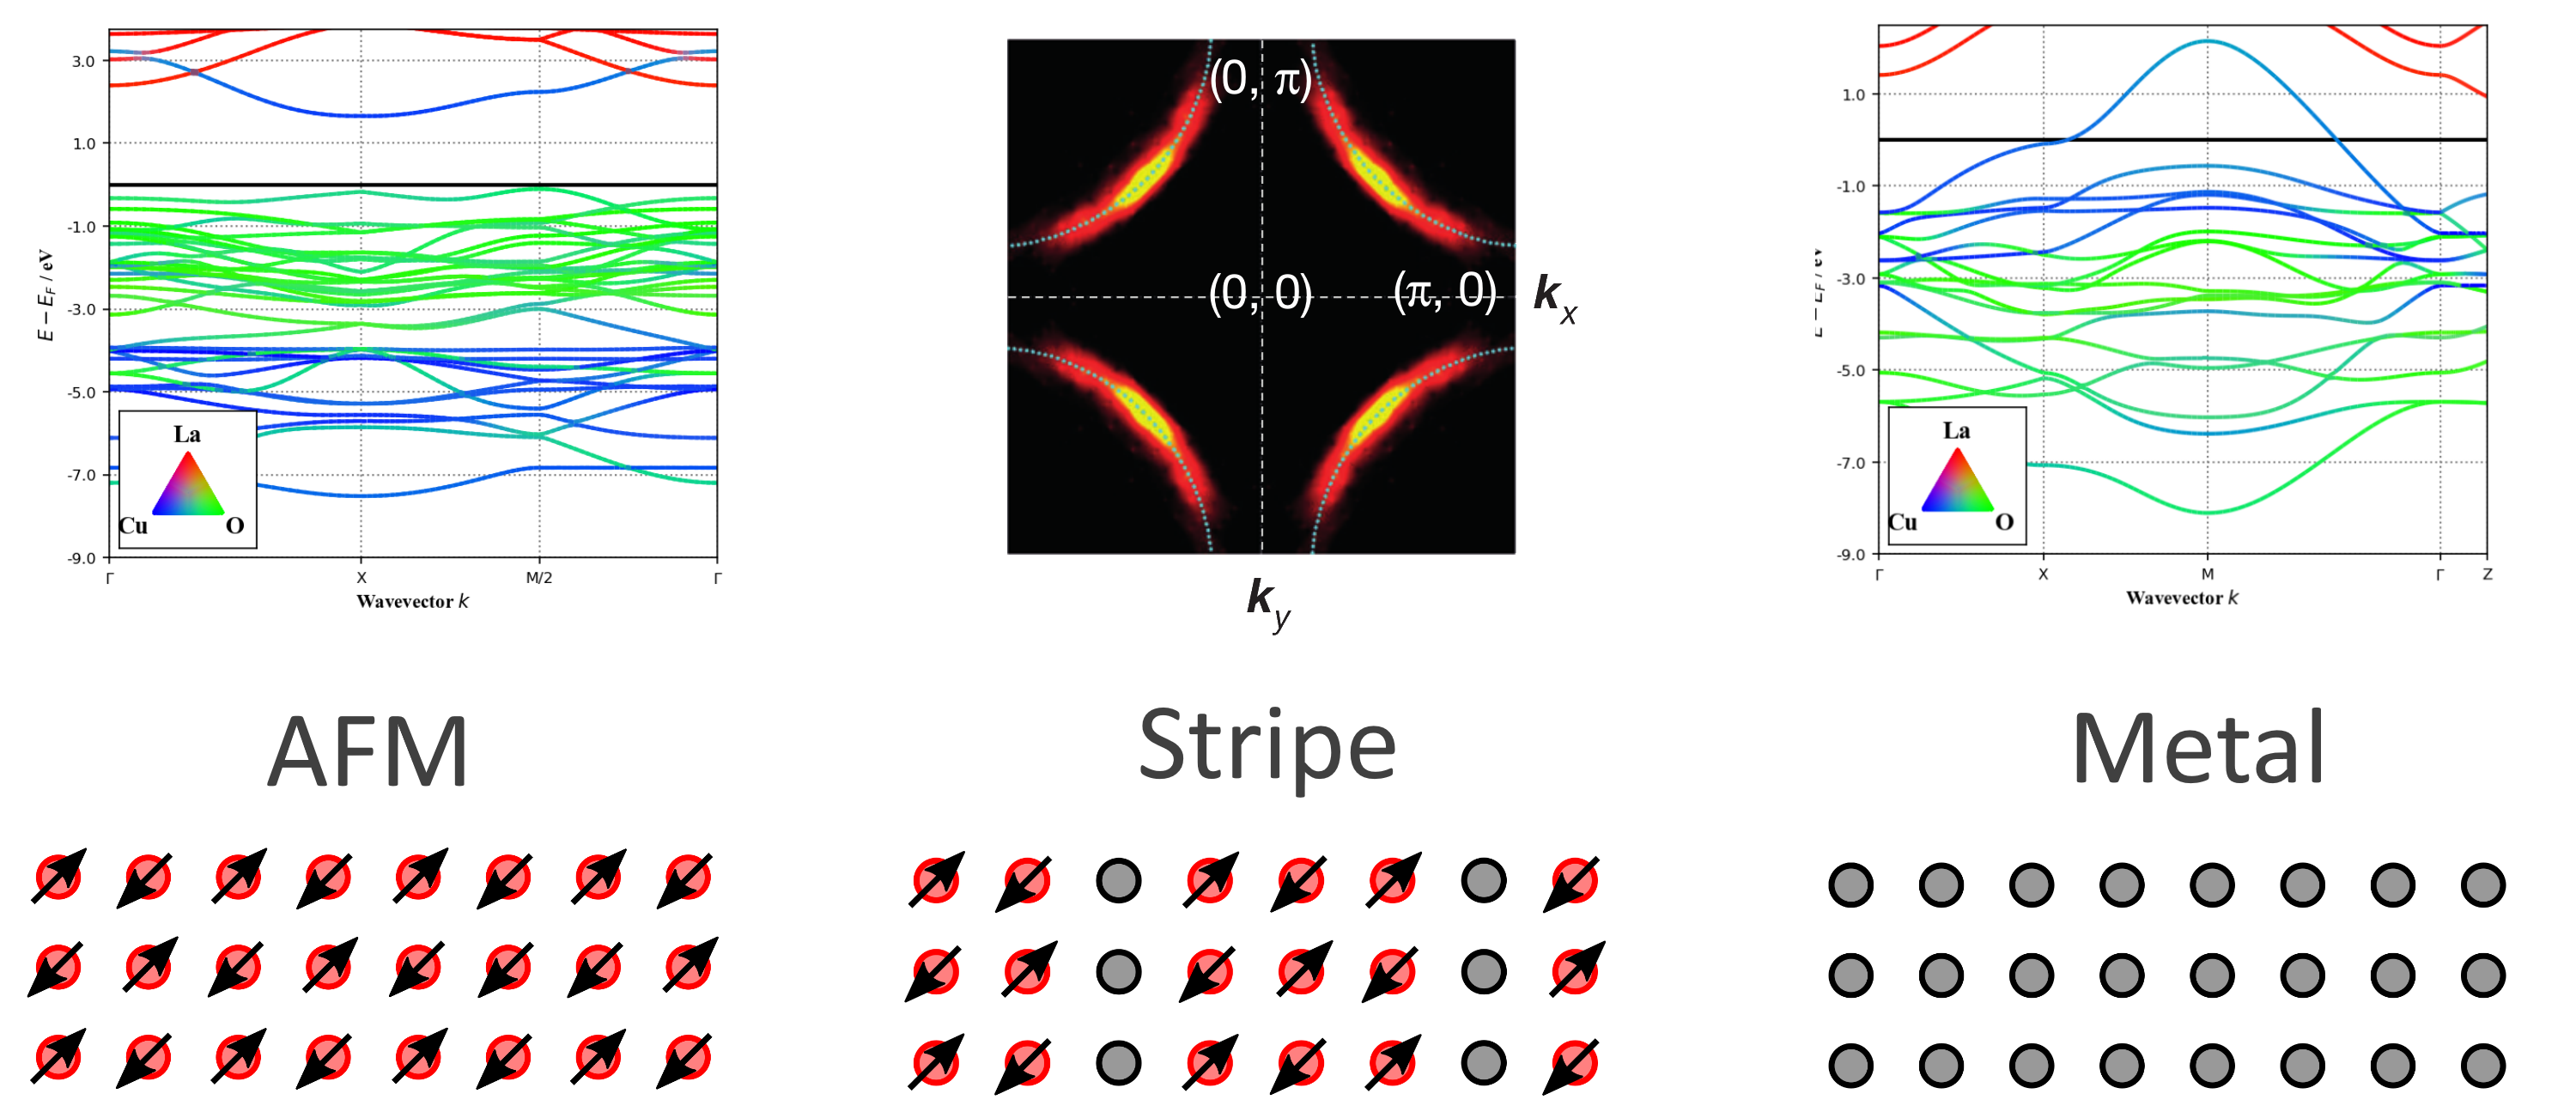
\includegraphics[width=\textwidth]{fig/conclusion/stripe_electronic_structure.png}
    \caption{Schematic of the electronic structure as a function of hole doping $n_\text{h}$. As one moves from left to right, $n_\text{h}$ increases. On the left we have the undoped compound where there is a gap in electronic density of states due to the antiferromagnetic ground state. As doping is increased, the strong antiferromagnetic interactions are disrupted and novel phenomena such as stripe order and broken Fermi arcs emerge \cite{Keimer2015}. Finally, on the right, the hole doping is sufficient such that the material becomes a normal metal and the strong correlations are destroyed. The electronic band structures are calculated and presented in chapter \ref{ch:simulation}.}
    \label{fig:conclusion_stripe_dft}
\end{figure}

Figure \ref{fig:conclusion_stripe_dft} attempts to visualize this problem by showing how superconductivity is squeezed between localized electrons giving rise to antiferromagnetic order and a fermi liquid with itinerant electrons and a continuous Fermi surface. The solution to this problem was to simply consider the two cases available to us and perform the calculations with this drawback in mind. In some sense, we are trying to figure out how well this level of theory can explain experimental observations. Exactly for this reason, I think a crucial part of this thesis is a careful evaluation of theory with experiment -- essentially we need to know `how wrong' the theory is.

Now, we are certainly not the first to consider La$_2$CuO$_4$ within a one-electron theory. Since DFT was well-established when the high-temperature superconductors were discovered, this methodology was applied right away (see review by \citeauthor{Pickett1989} \cite{Pickett1989}). Various levels of theory have applied to La$_2$CuO$_4$, including pure Hartree-Fock \cite{Su1999}, and semi-local potentials \cite{Lane2018}. Correlated phenomena, such as stripes \cite{Anisimov2004} and broken up Fermi arcs \cite{Lazic2015, Lazic2015a} have even been calculated within DFT, albeit with ad-hoc methods such as DFT+U. 

In this thesis, I make no attempt to contribute to this discussion. Rather, I prioritize getting accurate inter-atomic \emph{forces} such that we get the best possible representation of the phonon spectrum. We thus stick to the generally accepted GGA level of theory. As we saw in chapter \ref{ch:simulation}, some experimentation lead us to the PBESol functional and a significantly increased plane-wave cutoff in order to get reasonable acoustic phonons. 

Within this framework, it was possible to get a good description of the unstable modes related to the structural phase transitions observed in La$_2$CuO$_4$. However, it turns out that the low-temperature tetragonal (LTT) phase is the `most stable' structural phase both with respect to total energy and unstable phonons. Since this LTT phase is known to be suppressing superconductivity, our calculations are consistent with a picture where superconductivity competes with this structural phase and thus prevents the structural phase transition. In this context, I remark that the isostructural, non-superconducting compound La$_2$NiO$_4$ is LTT at low temperatures \cite{Tranquada1994}.

While more experimentation with structural phases, functionals and computational parameters is always desireable, I decided to move on with the relatively successful description of phonon dynamics in La$_2$CuO$_4$ within DFT. In chapter \ref{ch:md}, we use these simulations to approach the actual objective of treating doped La$_2$CuO$_4$ as a defect structure with molecular dynamics. Our analysis of the trajectories show that oxygen interstitials tend towards a LTT-like structure, while undoped and strontium-doped compounds stay LTO-like. While our simulation box and total simulation time is somewhat limited, these results is a good indication of \emph{distinct} dynamics associated with interstitials. Importantly, these distinct dynamics are associated with a modification of the phonon density-of-states which can be observed experimentally.

\section{Oxygen Interstitial Observables}
A large part of this thesis has been dedicated to finding signatures of oxygen interstitials. As mentioned in the introduction, these materials appear to optimize the superconducting transition temperature $T_\text{c}$ and it is suspected that the mobile, interstitial nature might be important for the elevated $T_\text{c}$. As we also show in chapter \ref{ch:local}, the `annealed doping' \cite{Wells1997} associated with interstitial oxygen is mainly observed in diffraction experiments. Remarkably, our high-quality PDF measurement shows almost no signature of oxygen interstitials. The superstructures observed in single-crystal measurements are so strong that this absence must be due to either rotational averaging or because powdered samples simply don't have these superstructures.

However, the dynamics of the \emph{same} powdered samples (measured in chapter \ref{ch:in4}) does have a signature of oxygen interstitials through a broadening of the phonon DOS in the \SIrange{10}{25}{\milli\eV} range. We can qualitatively identify this broadening, through our simulations, as a signature of oxygen disorder. In the case of strontium-doping, on the other hand, we see a sharpening of features which cannot be explained through our simulations. It is possible that the electronic structure of the LSCO $x=0.03$ sample modifies the phonon spectrum in a novel way, but more experiments are required to understand the observations. The fact that we can identify the features in this manner suggests that our model captures some of the dynamics associated with interstitials. This, in extension, is evidence for LTT-like tilts in La$_2$CuO$_{4+\delta}$ in a sample that is always observed to be structurally LTO.

This intimate relationship to an incipient tetragonal phase is also observed in our measurements of soft phonons in chapter \ref{ch:lowen}. While none of these measurements are conclusive on their own, taken together they point to LTT-like behavior being important in La$_2$CuO$_{4+\delta}$ (LCO+O). To briefly recap, I have found that LCO+O features

\begin{enumerate}
    \item LTT-like tilt dynamics.
    \item Instability towards LTT which is stabilized at $T_\text{c}$.
    \item Phase separation into distinct $n_\text{h}=\frac{1}{8}$ and optimally superconducting phases \cite{Mohottala2006,Udby2013}.
\end{enumerate}

\noindent Allowing myself to speculate wildly, this is consistent with a scenario where La$_2$CuO$_{4+\delta}$ is able to optimize the relationship between a stripe phase and a superconducting phase by leveraging LTT-like tilts. In this way, the annealed oxygen order, optimally superconducting phase can be `close' to the static stripe phase without actually being pinned by LTT symmetry. This is consistent with a situation where `stripe degrees of freedom' are necessary for superconductivity, but where we need to be sufficiently far away from static order. Essentially, one could think of a situation where the mobile dopants in La$_2$CuO$_{4+\delta}$ self-organize in a way that optimizes the conditions for these competing orders. A similar idea has been put forward by \citeauthor{Poccia2017} \cite{Poccia2017}, where it is suggested that grain boundaries help optimize this mechanism.

\section{Phonons and Stripes}
The relationship to stripe order in LCO+O was also investigated through measurements of the phonon anomaly in chapter \ref{ch:anomaly}. Contrary to what we saw in the preceding chapters, the phonon anomaly appears to be unrelated to the type of dopant or stripe order. In fact, when reviewing the samples where the phonon anomaly has been observed it appears to be a signature of doping $0.12 < n_\text{h} < 0.20$.

We interpret this as fluctuations of charge stripes, i.e. the stripe degrees of freedom mentioned above. Following the logic from before, this then suggests that charge fluctuations are a necessary but not sufficient condition for optimal superconductivity. In addition, the anomaly persists to high temperatures, so the phenomenon must be intrinsic to the doped samples in a large temperature range.

Very recently, resonant X-ray methods were used to determine `charge density fluctuations' (CDF) in samples of YBa$_2$Cu$_3$O$_{7-\delta}$ and Nd$_{1+x}$Ba$_{2-x}$Cu$_3$O$_{7-\delta}$ over a large doping range. Similar to what has been observed in the phonon anomaly, the CDF's are constrained in the phase diagram, but persists well above the pseudogap temperature $T^*$. Figure \ref{fig:cdw_summary} shows a summary of their results and a schematic of where one finds the phonon anomaly. The similarity of these phenomena strongly supports the suggested \cite{Reznik2012} connection between the phonon anomaly and dynamic stripes.

Finally, we discovered that the electronic structure as observed by ARPES in La$_2$CuO$_{4+\delta}$ is remarkably similar to that of overdoped La$_{1.77}$Sr$_{0.23}$CuO$_4$. Since La$_2$CuO$_{4+\delta}$ is known to phase separate into stripe ordered and superconducting phases, this is interpreted as a superposition of the two phenomena in the ARPES spectrum in chapter \ref{ch:arpes}

\begin{figure}
    \centering
    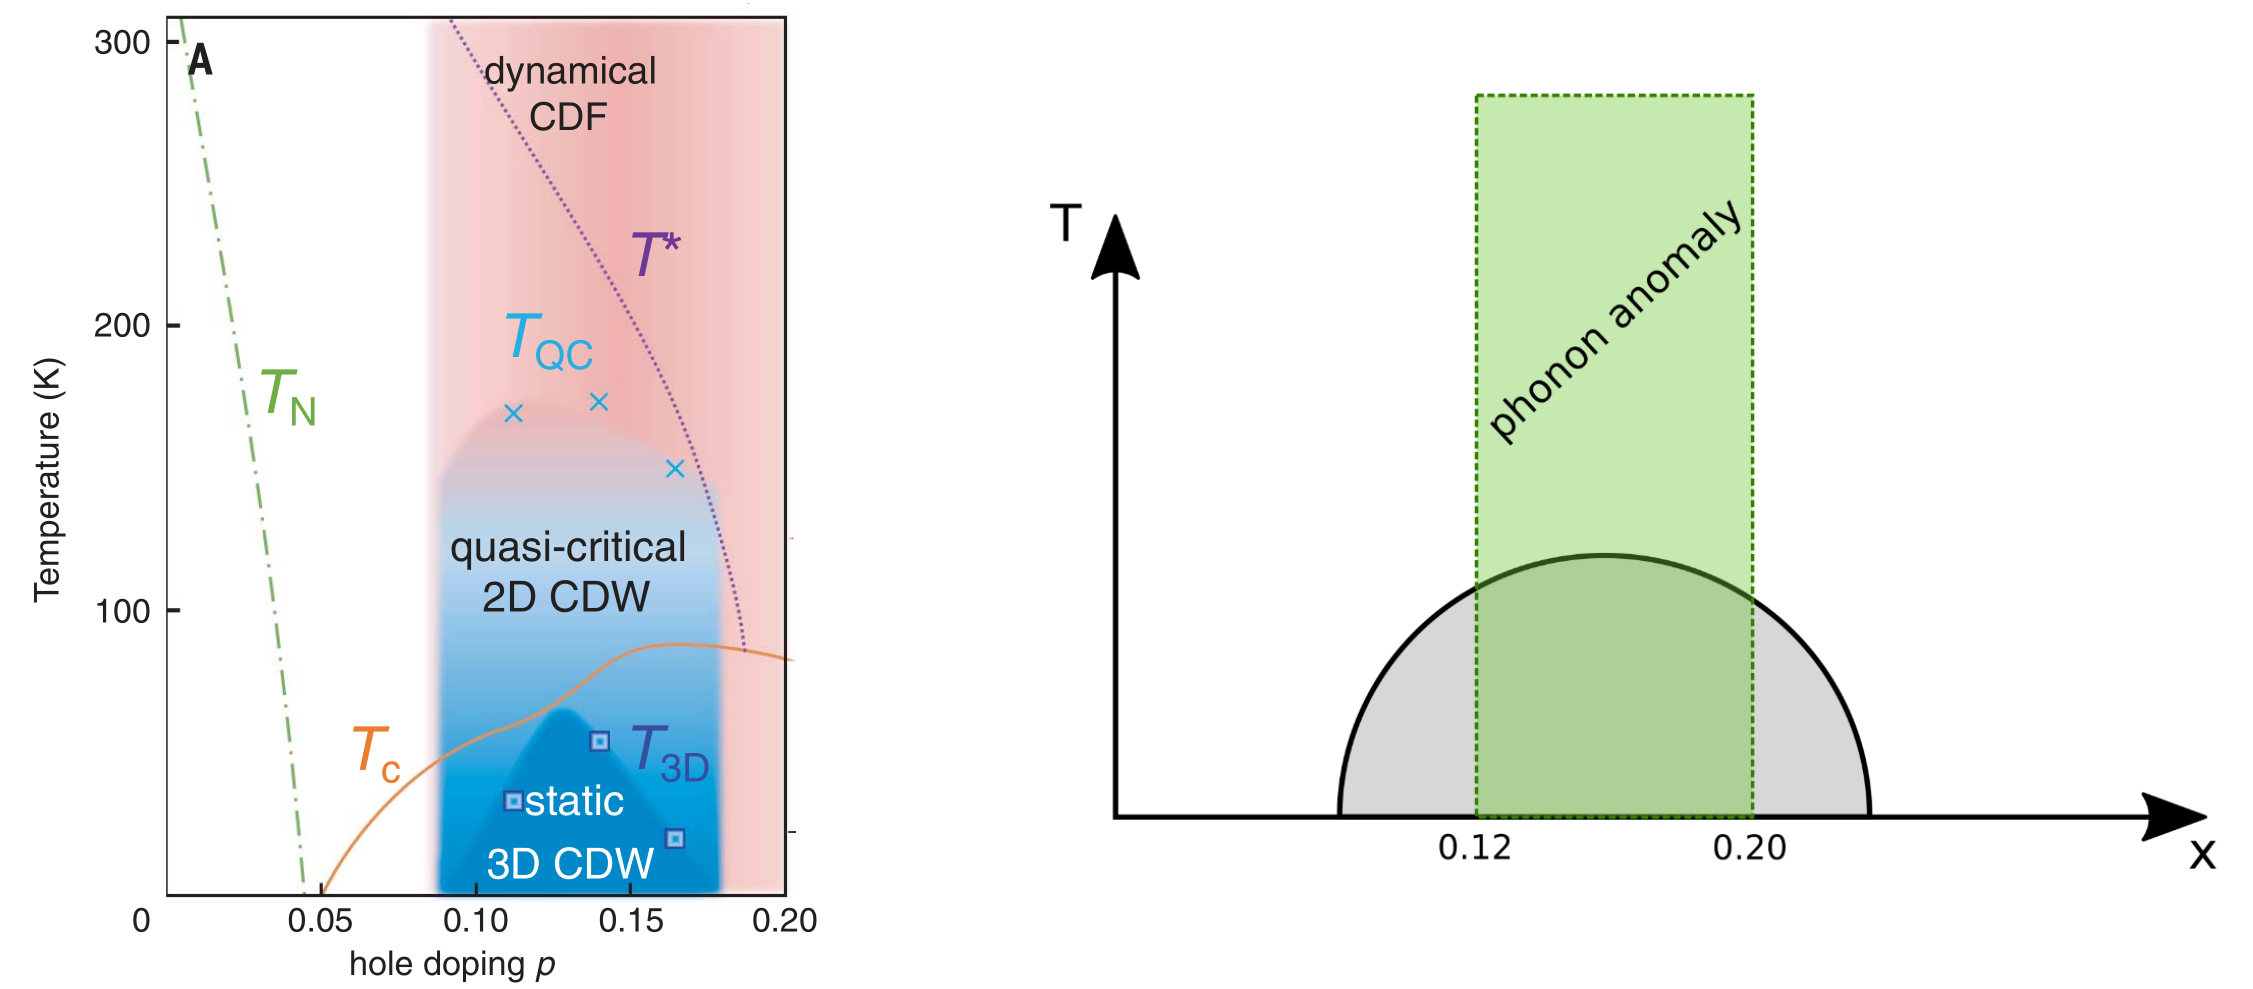
\includegraphics[width=\textwidth]{fig/conclusion/cdw_summary.png}
    \caption{\textbf{Left:} YBa$_2$Cu$_3$O$_{7-\delta}$ and Nd$_{1+x}$Ba$_{2-x}$Cu$_3$O$_{7-\delta}$ phase diagram showing charge fluctuations in a wide doping/temperature range \cite{Arpaia2019}. \textbf{Right:} Schematic of where the phonon anomaly appears in a generalized cuprate phase diagram (see dicussion in chapter \ref{ch:anomaly}).}
    \label{fig:cdw_summary}
\end{figure}

% \section{Outlook}
% In more concrete terms, I would propose the following research projects:

% \begin{enumerate}
%     \item An extended study of forces in Cuprates using DFT based on our results. Are there other functionals or higher-level theories that might be important in the evaluation of forces. Could include other cuprates to test for generality.
%     \item Classical molecular dynamics of LCO+O. Since DFT limits the size of our simulations box, it could be interesting to construct a large supercell and investigate if the observed superstructures emerge. Forces could be evaluated from the DFT calculations performed here.
%     \item A study of the observed superstructures in La$_2$CuO$_{4+\delta}$ and La$_2$NiO$_{4+\delta}$. Perhaps reverse monte-carlo methods or 2D PDF could be used to solve these structures.
% \end{enumerate}



